
Now that we have our benchmarking code to measure the speed of reading and writing into memory, we can collect the results and see how we can get the best performance when accessing data in memory. We begin with random access, where the location of each value we read or write is unpredictable.



\subsubsubsection{4.4.1\hspace{0.2cm}The speed of random memory access}

The measurements are likely to be fairly noisy unless you run this benchmark many times and average the results (the benchmark library can do that for you). For a reasonable run time (minutes), you will likely see the results that look something like this:

\hspace*{\fill} \\ %插入空行
\begin{center}
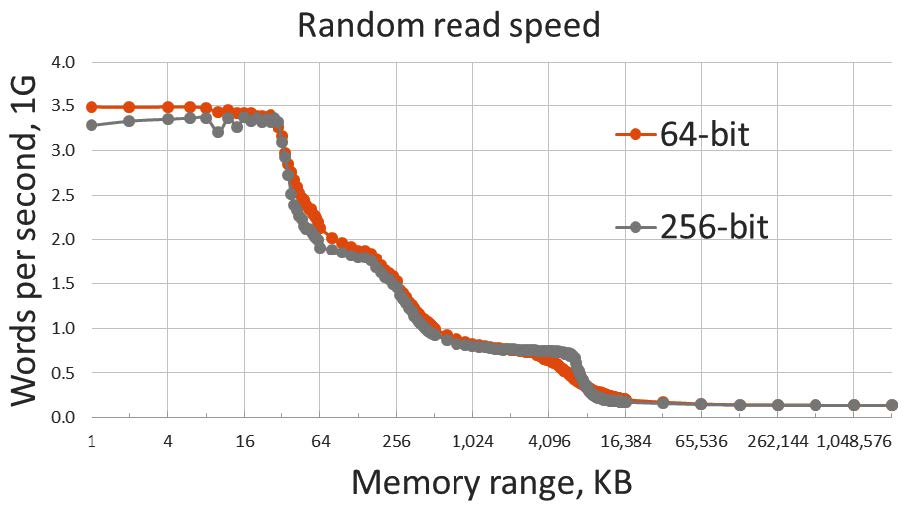
\includegraphics[width=0.9\textwidth]{content/1/chapter4/images/3.jpg}\\
Figure 4.3 – Random read speed as a function of memory size
\end{center}

The benchmark results in Figure 4.3 show the number of words read from memory per second (in billions, on any reasonable PC or workstation you can find today), where the word is a 64-bit integer or a 265-bit integer (long or \_\_m256i, respectively). The same measurements can be alternatively presented as the time it takes to read a single word of the chosen size:

\hspace*{\fill} \\ %插入空行
\begin{center}
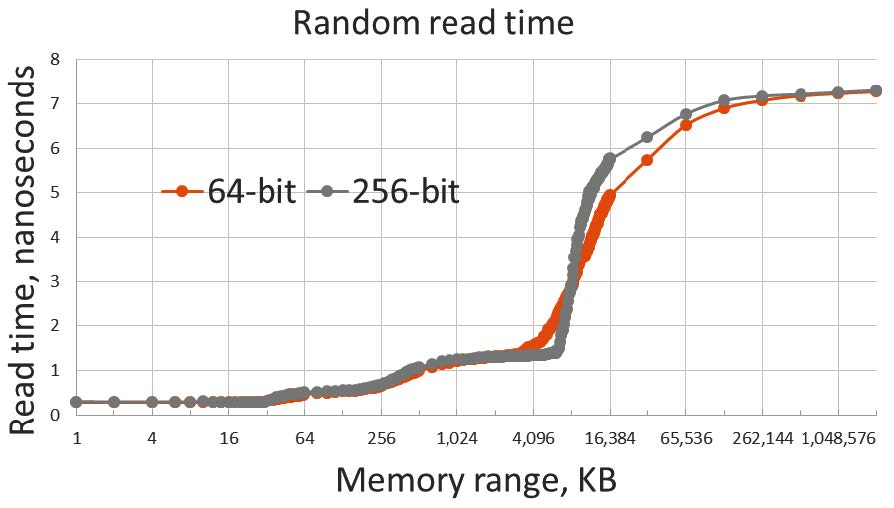
\includegraphics[width=0.9\textwidth]{content/1/chapter4/images/4.jpg}\\
Figure 4.4 – Read time for one array element versus array size
\end{center}

The graphs have several interesting features we can observe at once. First of all, as we expected, there is no single memory speed. The time it takes to read a single 64-bit integer varies from 0.3 nanoseconds to 7 nanoseconds on the machine I have used. Reading small amounts of data is significantly faster, per value, than reading large amounts of data. We can see the cache sizes in these graphs: the L1 cache of 32 KB is fast, and the read speed does not depend on the data volume as long as it all fits into the L1 cache. As soon as we exceed 32 KB of data, the read speed starts to drop. The data now fits into the L2 cache, which is larger (256 KB) but slower. The larger the array, the smaller is the portion of it that fits into the fast L1 cache at any time, and the slower is the access.

The read time increases even more if the data spills out of the L2 cache, and we have to use the L3 cache, which is even slower. The L3 cache is much larger, though, so nothing happens until the data size exceeds 8 MB. Only at that point do we actually start reading from the main memory: until now, the data was moved from the memory into caches the first time we touched it, and all subsequent read operations used the caches only. But if we need to access more than 8 MB of data at once, some of it will have to be read from the main memory (on this machine, anyway—cache sizes vary between CPU models). We don't lose the benefit of caches right away, of course: as long as most data fits in the cache, it is at least somewhat effective. But once the volume of data exceeds the cache size by several times, the read time is almost completely determined by the time it takes to retrieve the data from the memory. 

Whenever we need to read or write some variable, and we find it in a cache, we call it a cache hit. However, if it's not found, then we register a cache miss. Of course, an L1 cache miss can be an L2 hit. An L3 cache miss means that we have to go all the way to the main memory.

The second property of note is the value itself: 7 nanoseconds to read a single integer from memory. By processor standards, this is a very long time: in the previous chapter, we have seen that the same CPU can do several operations per nanosecond. Let this sink in: the CPU can do about 50 arithmetic operations in the time it takes to read a single integer value from memory unless the value happens to be in the cache already. Very few programs need to do 50 operations on each value, which means that the CPU will likely be underutilized unless we can figure out something to speed up memory access.

Finally, we see that the read speed in words per second does not depend on the size of the word. From a practical point of view, the most relevant implication is that we can read four times as much data if we use 256-bit instructions to read the memory. Of course, it's not that simple: SSE and AVX load instructions read values into different registers than the regular loads, so we also have to use the SSE or AVX SIMD instructions to do the computations. One simpler case is when we just need to copy a large amount of data from one location in memory to another; our measurements suggest that copying 256-bit words does the job four times faster than using 64-bit words. Of course, there is already a library function that copies memory, memcpy() or std::memcpy(), and it is optimized for best efficiency.

There is another implication from the fact that the speed does not depend on the word size: it implies that the read speed is limited by latency and not by bandwidth. Latency is the delay between the time the request for data is issued and the time the data is retrieved. Bandwidth is the total amount of data the memory bus can transmit in a given time. Going from a 64-bit word to a 256-bit word transmits four times as much data in the same time; this implies that we haven't hit the bandwidth limit yet. While this may seem like a purely theoretical distinction, it does have important consequences for writing efficient programs that we will learn about later in this chapter.

Finally, we can measure the speed of writing the memory:

\hspace*{\fill} \\ %插入空行
\begin{center}
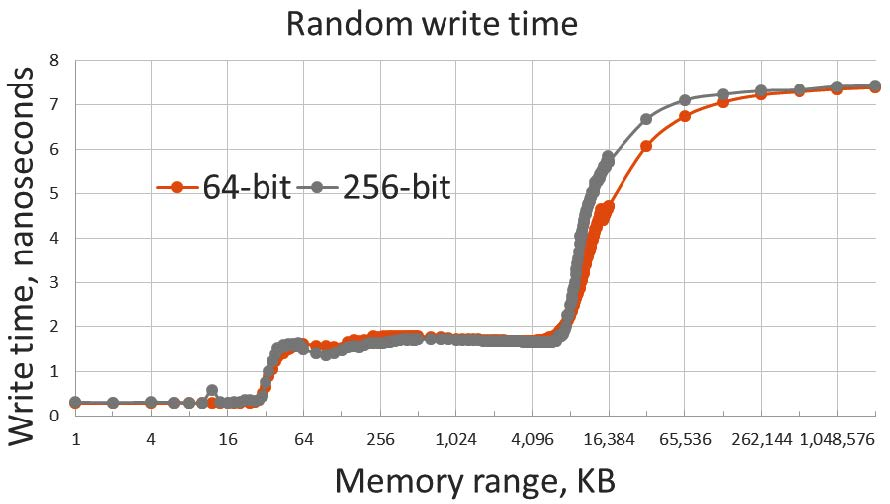
\includegraphics[width=0.9\textwidth]{content/1/chapter4/images/5.jpg}\\
Figure 4.5 – Write time for one array element versus array size
\end{center}

In our case, the random reads and writes have very similar performance, but this can vary for different hardware: sometimes reads are faster. Everything we observed earlier about the speed of reading memory also applies to writing: we see the cache size effects in Figure 4.5, the overall wait time for a write is very long if the main memory is involved, and writing large words is more efficient.

What can we conclude about the impact of memory access on performance? On the one hand, if we need to access a small amount of data (less than 32 KB) repeatedly, we don't have to worry much about it. Of course, repeatedly is the key here: the first access to any memory location will have to touch the main memory regardless of how much memory we plan to access (the computer doesn't know that your array is small until you read the entire array and go back to the beginning—reading the first element of a small array for the first time looks exactly the same as reading the first element of a large array). On the other hand, if we have to access large amounts of data, the memory speed is likely to become our first concern: at 7 nanoseconds per number, you can't get very far.

There are several techniques for improving memory performance that we will see throughout this chapter. Before we study how to improve our code, let us see what help we can get from the hardware itself.

\subsubsubsection{4.4.2\hspace{0.2cm}The speed of sequential memory access}

So far, we have measured the speed of accessing memory at random locations. When we do this, every memory access is effectively new. The entire array we are reading is loaded into the smallest cache it can fit into, and then our reads and writes randomly access different locations in that cache. If the array does not fit into any cache, then we randomly access different locations in memory and incur the 7 nanoseconds latency on every access (for the hardware we use).

Random memory accesses happen quite often in our programs, but just as often, we have a large array that we need to process from the first element to the last. It is important to point out that random and sequential access here is determined by the order of memory addresses. There is a potential for misunderstanding: a list is a data structure that does not support random access (meaning you cannot jump into the middle of the list) and must be accessed sequentially, starting from the head element. However, traversing the list sequentially is likely to access the memory in random order if each list element was allocated separately and at different times. An array, on the other hand, is a random access data structure (meaning you can access any element without accessing the ones before it). However, reading the array from the beginning to the end accesses memory sequentially, in order of monotonically increasing addresses. In this entire chapter, unless otherwise stated, we are concerned with the order of accessing memory addresses when we talk about sequential or random access.

The performance of sequential memory accesses is quite different. Here are the results for sequential writes:

\hspace*{\fill} \\ %插入空行
\begin{center}
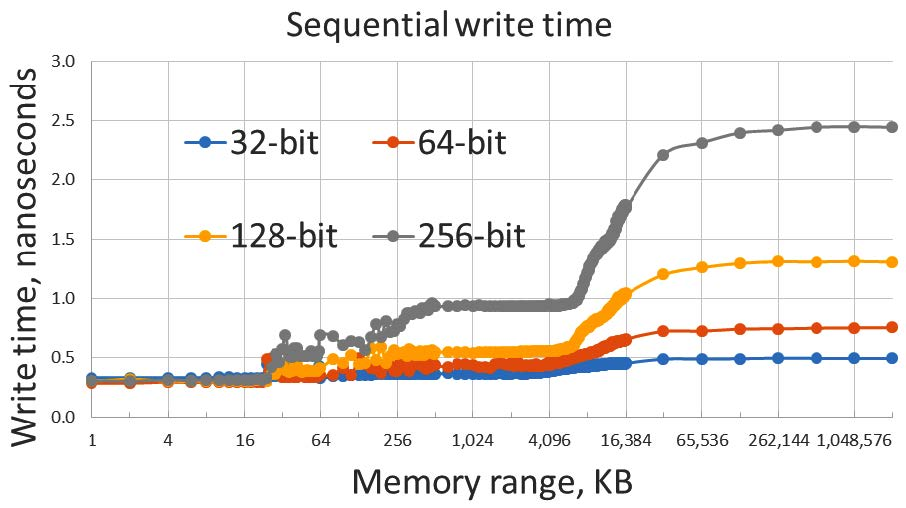
\includegraphics[width=0.9\textwidth]{content/1/chapter4/images/6.jpg}\\
Figure 4.6 – Write time for one array element versus array size, sequential access
\end{center}

The overall shape of the graphs is the same as before, but the differences are just as important as the similarities. The first difference we should note is the scale of the vertical axis: the time values are much smaller than the ones we saw in Figure 4.5. It takes only 2.5 nanoseconds to write a 256-bit value and just 0.8 nanoseconds for the 64-bit integer.

The second difference is that the curves for different word sizes are no longer the same. An important caveat here is that this result is highly hardware-dependent: on many systems, you will see the results more similar to the ones from the previous section. On the hardware I used, sequential write times for different word sizes are the same for the L1 cache but different for other caches and the main memory. Looking at the main memory values, we can observe that the time to write a 64-bit integer is not quite twice the time it takes to write a 32-bit integer, and for the larger sizes, the write times double every time the word size doubles. This means that the limit is not how many words per second we can write, but how many bytes per second: the speed in bytes per second will be the same for all word sizes (except the smallest one). This implies that the speed is now limited not by latency but by bandwidth: we're pushing the bits into memory as fast as the bus can transmit them, and it doesn't matter whether we group them into 64-bit chunks or 256-bit chunks that we call words, we've hit the bandwidth limit of the memory. Again, this outcome is much more hardware-dependent than any other observation we make in this chapter: on many machines, the memory is fast enough, and a single CPU cannot saturate its bandwidth.

The last observation we can make is that while the steps in the curves corresponding to the cache sizes are still visible, they are much less pronounced and not nearly as steep. We have the results, we have the observations. What does this all mean?


\subsubsubsection{4.4.3\hspace{0.2cm}Memory performance optimizations in hardware}

The three observations, combined, point to some sort of latency-hiding technique employed by the hardware itself (other than changing the memory access order, we have not done anything to improve the performance of our code, so the gains are all thanks to the hardware doing something different). When accessing the main memory randomly, each access takes 7 nanoseconds on our machine. That's how long it takes from the time the data at a particular address is requested until it's delivered into a CPU register, and this delay is entirely determined by latency (it doesn't matter how many bytes we requested, we have to wait for 7 nanoseconds to get anything). When accessing memory sequentially, the hardware can begin transferring the next element of the array right away: the very first element still takes 7 nanoseconds to access, but after that, the hardware can start streaming the entire array from or to memory as fast as the CPU and the memory bus can handle it. The transfer of the second and the later elements of the array begins even before the CPU has issued the request for the data. Thus, the latency is no longer the limiting factor, the bandwidth is.

Of course, this assumes that the hardware knows that we want to access the entire array sequentially and how large the array is. In reality, the hardware knows nothing of the sort, but, just like it did with the conditional instructions we studied in the last chapter, there are learning circuits in the memory system that make educated guesses. In our case, we have encountered the hardware technique known as the prefetch. Once the memory controller notices that the CPU has accessed several addresses sequentially, it makes the assumption that the pattern will continue and prepares for the access of the next memory location by transferring the data into the L1 cache (for reads) or vacating space in the L1 cache (for writes). Ideally, the prefetch technique would allow the CPU always to access memory at the L1 cache speeds because, by the time the CPU needs each array element, it is already in the L1 cache. Whether the reality matches this ideal case or not depends on how much work the CPU needs to do between accessing the adjacent elements. In our benchmark, the CPU does almost no work at all, and the prefetch falls behind. Even anticipating the linear sequential access, there is no way it can transfer the data between the main memory and the L1 cache fast enough. However, the prefetch is very effective at hiding the latency of memory access.

The prefetch is not based on any prescience or prior knowledge about how the memory is going to be accessed (there are some platform-specific system calls that allow the program to notify the hardware that a range of memory is about to be accessed sequentially, but they are not portable and, in practice, rarely useful). Instead, the prefetch tries to detect a pattern in accessing memory. The effectiveness of the prefetch is, thus, determined by how effectively it can determine the pattern and guess the location of the next access.

There is a lot of information, much of it is outdated, about what the limitations of the prefetch pattern detection are. For example, in the older literature, you can read that accessing memory in the forward order (for an array a, going from a[0] to a[N-1]) is more efficient than going backward. This is no longer true for any modern CPU and hasn't been true for years. This book risks falling into the same trap if I start describing exactly which patterns are and aren't efficient in terms of prefetch. Ultimately, if your algorithm requires a particular memory access pattern and you want to find out whether your prefetch can handle it, the most reliable way is to measure it using the benchmark code similar to what we used in this chapter for random memory access.

In general terms, I can tell you that the prefetch is equally effective for accessing memory in increasing and decreasing orders. However, reversing the direction will incur some penalty until the prefetch adjusts to the new pattern. Accessing memory with stride, such as accessing every fourth element in an array, will be detected and predicted just as efficiently as a dense sequential access. The prefetch can detect multiple concurrent strides (that is, accessing every third and every seventh element), but here we're getting into the territory where you have to gather your own data as the hardware capabilities change from one processor to another.

Another performance optimization technique that the hardware employs very successfully is the familiar one: pipelining or hardware loop unrolling. We have already seen it in the last chapter, where it was used to hide the delay caused by the conditional instructions. Similarly, pipelining is used to hide the latency of memory accesses. Consider this loop:

\begin{lstlisting}[style=styleCXX]
for (size_t i = 0; i < N; ++i) {
	b[i] = func(a[i]);
}
\end{lstlisting}

On every iteration, we read a value a[i] from the array, do some computations, and store the result, b[i], in another array. Since both reading and writing takes time, we can expect the timeline of the execution of the loop to look like this:

\hspace*{\fill} \\ %插入空行
\begin{center}
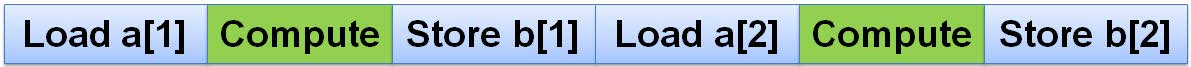
\includegraphics[width=0.9\textwidth]{content/1/chapter4/images/7.jpg}\\
Figure 4.7 – Timeline of a non-pipelined loop
\end{center}

This sequence of operations would leave the CPU waiting for memory operations to complete most of the time. Instead, the hardware will read ahead into the instruction stream and overlay the instruction sequences that do not depend on each other:

\hspace*{\fill} \\ %插入空行
\begin{center}
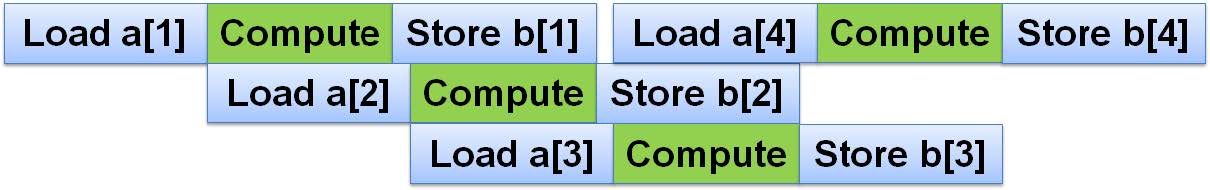
\includegraphics[width=0.9\textwidth]{content/1/chapter4/images/8.jpg}\\
Figure 4.8 – Timeline of a pipelined (unrolled) loop
\end{center}

The load of the second array element can start as soon as the first one is read, assuming there are enough registers. For simplicity, we are assuming that the CPU cannot load two values at a time; most real CPUs can do more than one memory access at the same time, which just means that the pipeline can be even wider, but it doesn't change the main idea. The second set of computations begin as soon as the input value is available. After the first few steps, the pipeline is loaded, and the CPU spends most of the time computing (if the computing steps from different iterations overlap, the CPU may even be executing several iterations at once, provided it has enough compute units to do so).

The pipelining can hide the latency of memory accesses, but, obviously, there is a limit. If it takes 7 nanoseconds to read one value and we need to read a million of them, it is going to take 7 milliseconds at best, there is no getting around that (again, assuming the CPU can read only one value at a time). The pipelining can help us by overlaying the computations with the memory operations, so, in the ideal case, all the computing is done during these 7 milliseconds. The prefetch can start reading the next value before we need it and thus cut down the average read time, but only if it guesses correctly what that value is. Either way, the measurements done in this chapter show the best-case scenarios for accessing memory in different ways.

In terms of measuring memory speed and presenting the results, we have covered the basics and learned about the general properties of the memory system. Any more detailed or specific measurements are left as an exercise for the reader, and you should be wellequipped to gather the data you need to make informed decisions about the performance of your particular applications. We now turn our attention to the next step: we know how the memory works and what performance we can expect from it, but what can we do to improve the performance of a concrete program?
















